\documentclass[11pt,twoside,a4paper]{article}
% http://www-h.eng.cam.ac.uk/help/tpl/textprocessing/latex_maths+pix/node6.html symboles de math
% http://fr.wikibooks.org/wiki/Programmation_LaTeX Programmation latex (wikibook)
%=========================== En-Tete =================================
%--- Insertion de paquetages (optionnel) ---
\usepackage[french]{babel}   % pour dire que le texte est en fran{\'e}ais
\usepackage{a4}	             % pour la taille   
%% \usepackage[T1]{fontenc}     % pour les font postscript
%% \usepackage{lmodern}
\usepackage{epsfig}          % pour gerer les images
\usepackage{amsmath, amsthm} % tres bon mode mathematique
\usepackage{amsfonts,amssymb}% permet la definition des ensembles
\usepackage{float}           % pour le placement des figures
\usepackage{verbatim}

\usepackage{longtable} % pour les tableaux de plusieurs pages

\usepackage[table]{xcolor} % couleur de fond des cellules de tableaux

\usepackage{lastpage}

\usepackage{lscape} % changement orientation page

\usepackage{tikz}
\usetikzlibrary{decorations.pathmorphing, shapes}

%% \setmainfont[Ligatures=TeX]{Computerfont}
\usepackage{fontspec}
\defaultfontfeatures{Mapping=tex-text,Scale=MatchLowercase}
\setmainfont{Ubuntu Mono} 
%% \setmainfont{Cyberpunk Is Not Dead}
%% \setmonofont{Lucida Sans Typewriter}

\usepackage[top=1.5cm, bottom=1.5cm, left=1.5cm, right=1.5cm]{geometry}
% gauche, haut, droite, bas, entete, ente2txt, pied, txt2pied
%% \usepackage{vmargin}
%% \setmarginsrb{1.0cm}{0.5cm}{1.0cm}{0.5cm}{15pt}{3pt}{60pt}{20pt}

%\usepackage{frbib} % enlever pour obtenir references en anglais
% --- style de page (pour les en-tete) ---
% \pagestyle{headings}

\def\magazineTitle{The Daily Timer}

\usepackage{lipsum} 

\usepackage{multicol} % pour {\'e}crire dans certaines zones en colonnes : \begin{multicols}{nb colonnes}...\end{multicols}

% % % en-tete et pieds de page configurables : fancyhdr.sty
% http://www.trustonme.net/didactels/250.html
% http://ww3.ac-poitiers.fr/math/tex/pratique/entete/entete.htm
% http://www.ctan.org/tex-archive/macros/latex/contrib/fancyhdr/fancyhdr.pdf
\usepackage{fancyhdr}
\pagestyle{fancy}
\fancyhf{}
\fancyhead[LE,RO]{\bfseries\thepage}
\fancyhead[LO]{\bfseries\rightmark}
\fancyhead[RE]{\bfseries\leftmark}
\fancyfoot[LE]{\thepage /\pageref{LastPage} \hfill
	\textbf{\magazineTitle }
\hfill 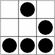
\includegraphics[width=0.5cm]{../logo_glider.png} }
\fancyfoot[RO]{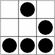
\includegraphics[width=0.5cm]{../logo_glider.png} \hfill
	\textbf{\magazineTitle }
\hfill \thepage /\pageref{LastPage}}
\renewcommand{\headrulewidth}{0.5pt}
\renewcommand{\footrulewidth}{0.5pt}
\addtolength{\headheight}{0.5pt}
\fancypagestyle{plain}{
	\fancyhead{}
	\fancyfoot{}
	\renewcommand{\headrulewidth}{0pt}
}

%--- Definitions de nouvelles commandes ---

%--- Pour le titre ---
\def\maketitle{%
	\setlength{\parindent}{0em}
	\begin{center}
		\begin{tabular}[c]{c|c|c}
								& \setmainfont{Young 20s} \Huge{The Daily Timer}		&			\\
								& 														&			\\
			Issue 0, Volume 0 	& \setmainfont{Young 20s} \Large{Street \& CyberPunk}	& \today	\\
								& 														&			\\
								& Nouvelles de Neo-Paris								&			\\
		\end{tabular}~\\
	\end{center}
	\setlength{\parindent}{2\parskip}
}%

%============================= Corps =================================
\begin{document}

% ecrire le titre...
\maketitle
\thispagestyle{empty}

\huge{\setmainfont{Cyberpunk Is Not Dead} Explosion du Hidenburg II : Militech Impliquée !}

\begin{multicols}{2}

\lipsum[5]

%% \vfill~\\ \columnbreak

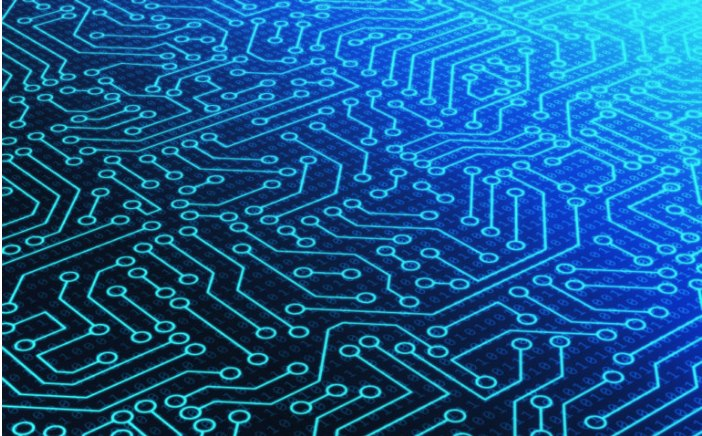
\includegraphics[width=0.50\textwidth]{../../images/62129055_10219405317945563_2140020562502615040_n.jpg}

\lipsum[3-4]

\vfill~\\ \columnbreak

	\begin{multicols}{2}
	
	\lipsum[1]
	
	\end{multicols}

\end{multicols}

\clearpage

%% le contenu

		\begin{minipage}[ht]{0.45\textwidth}
			\colorbox{purple!30}{
			\begin{tikzpicture}
				\draw[fill, gray] (0,0) arc (0:-180:1cm);
				\draw[fill, black] (0,0) arc (0:180:1cm);
				
				\draw[fill, red] 	(-1.25,-0.25) rectangle (-1.60,-5);
				\draw[fill, green] 	(-0.75,-0.25) rectangle (-1.10,-6);
				\draw[fill, blue] 	(-0.25,-0.25) rectangle (-0.60,-7);
			\end{tikzpicture}
			}
		\end{minipage}

%% https://tex.stackexchange.com/questions/474155/a0-hexagon-background-tikz
\def\hexapavage{--++(60:1)--+(120:1)++(0,0)--++(1,0)--++(60:1)--+(1,0)++(-120:1)--++(-60:1)}
\begin{tikzpicture}
	% PavageHexa avec scale
	\begin{scope}[yshift=-6cm,scale=.6]
		 \foreach \j in {0,1,...,3} {
			\foreach \i in {0,1,...,5} {
				\draw[thick] (60:\j)++(120:\j)++
				(60:\i)++(-60:\i)++(\i,0)++(\i,0) \hexapavage ;
	}}
	\draw[blue,very thick](0,0)\hexapavage;
	\end{scope}
\end{tikzpicture} 

\clearpage

\section{Section}

\subsection{Sous-section}

\subsubsection{sous sous sous section}

[...]~\\

\subsubsection{sous sous sous section}


\clearpage

\section*{Bibliographie\markboth{Bibliographie}{Bibliographie}}

\addcontentsline{toc}{section}{Bibliographie}
\nocite{*}
%toutes references biblio : 6 lettres + 2 chiffres
\bibliography{modele_journal1}
\bibliographystyle{frplain} % plain or frplain

\tableofcontents

\listoffigures

\listoftables

\end{document}
